The validation of the maximum likelihood fit, used to extract all information in this
analysis, is now described. The validation procedure consists of
two main tests. The first test is a fit using a data sample without
anomalous couplings. Such a test allows to identify problems with
event generation causing discrepancies in the leading lepton
\pt\ distribution. The second test is a fit using a data sample with
anomalous couplings. Such a test checks if we can properly measure
anomalous couplings when they are present. Both tests are critical to
validate the fitting tools, which are fairly complicated.

In the previous analysis it was found that the leading lepton
\pt\ distribution does not allow to differentiate between different
couplings and a typical observation inconsistent with Standard Model
represents a class of possible coupling values.

Figure~\ref{fig:val_scans} shows fit results and likelihood scans for
\ww\ simulated data with and without anomalous couplings. One may
conclude that even though the fit was able to measure the couplings
close to the true values, there is large uncertainty on the angle
between the two couplings as is revealed in the shapes of the contour
plots in the likelihood scans.

\begin{figure}[tp]
  \centerline{
    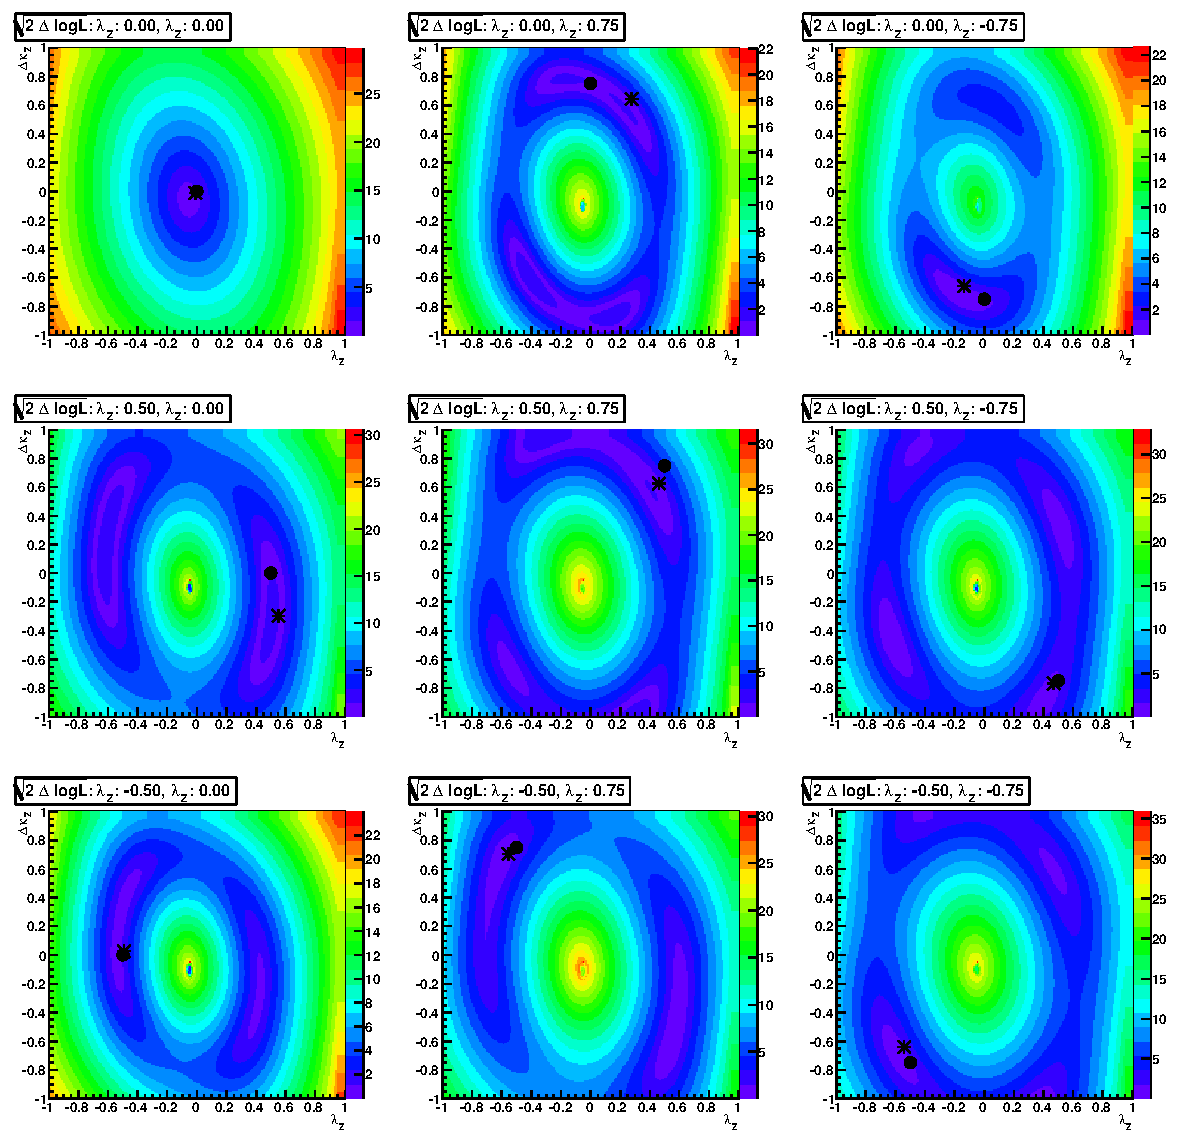
\includegraphics[width=1.0\textwidth]{figures/validation_likelihood_scans}
  }

  \caption[Likelihood scan for Signal Monte Carlo] {Likelihood scans
    for 350/pb of data excluding backgrounds. The curves
    represent the $\sqrt{2\Delta\log L}$ 1D significance of the difference between the
    likelihood with the sample's true anomalous couplings and the other
    values on the plain. The black star is the fit result when both couplings are
    allowed to float in the fit. The black point is the true value of the couplings.}
  \label{fig:val_scans}
\end{figure}

\subsection{Pseudo-experiments}
Figures~\ref{fig:fit_ww_mc_1D} and \ref{fig:fit_wwATGC_mc_1D_abs} show
results of the fits on \ww\ Monte Carlo samples with and without
anomalous couplings and excluding backgrounds. If only one coupling is
fitted it is not possible to get the sign right, so only absolute
values can be measured.

Pseudo-experiments with Standard Model \ww\ Monte Carlo are performed to look
for bias in the fit for the central value and to test the uncertainty
estimation. No significant deviation from zero is
found. Pseudo-experiments with non-zero anomalous couplings underestimate 
the true value by 20-30\%. To take this effect into
account we rescale final results.

\begin{figure}[tp]
  \centering
    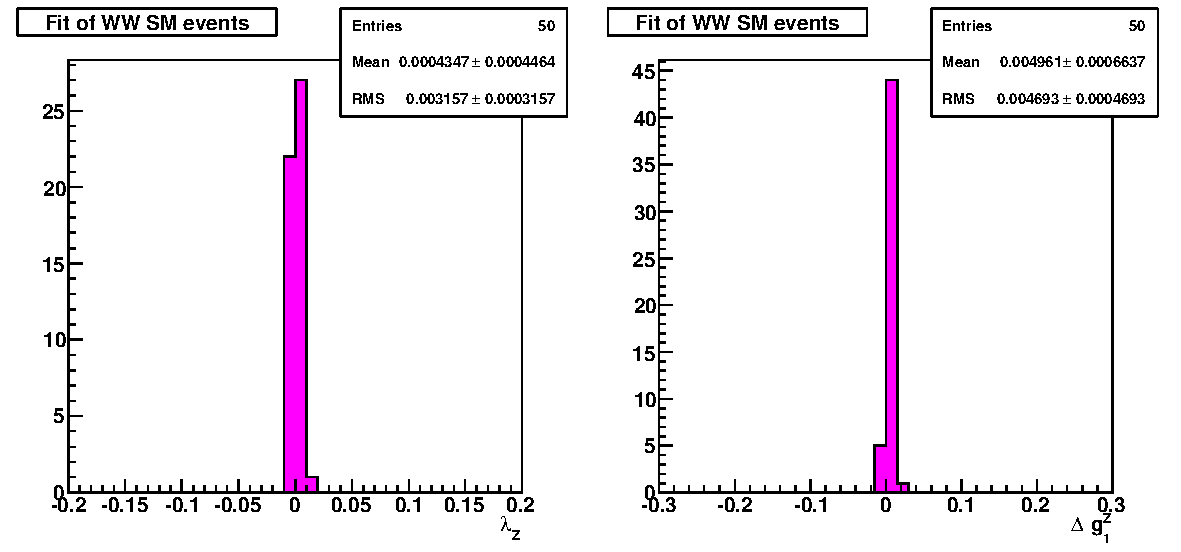
\includegraphics[width=1.0\textwidth]{figures/fit_ww_mc_1D}
    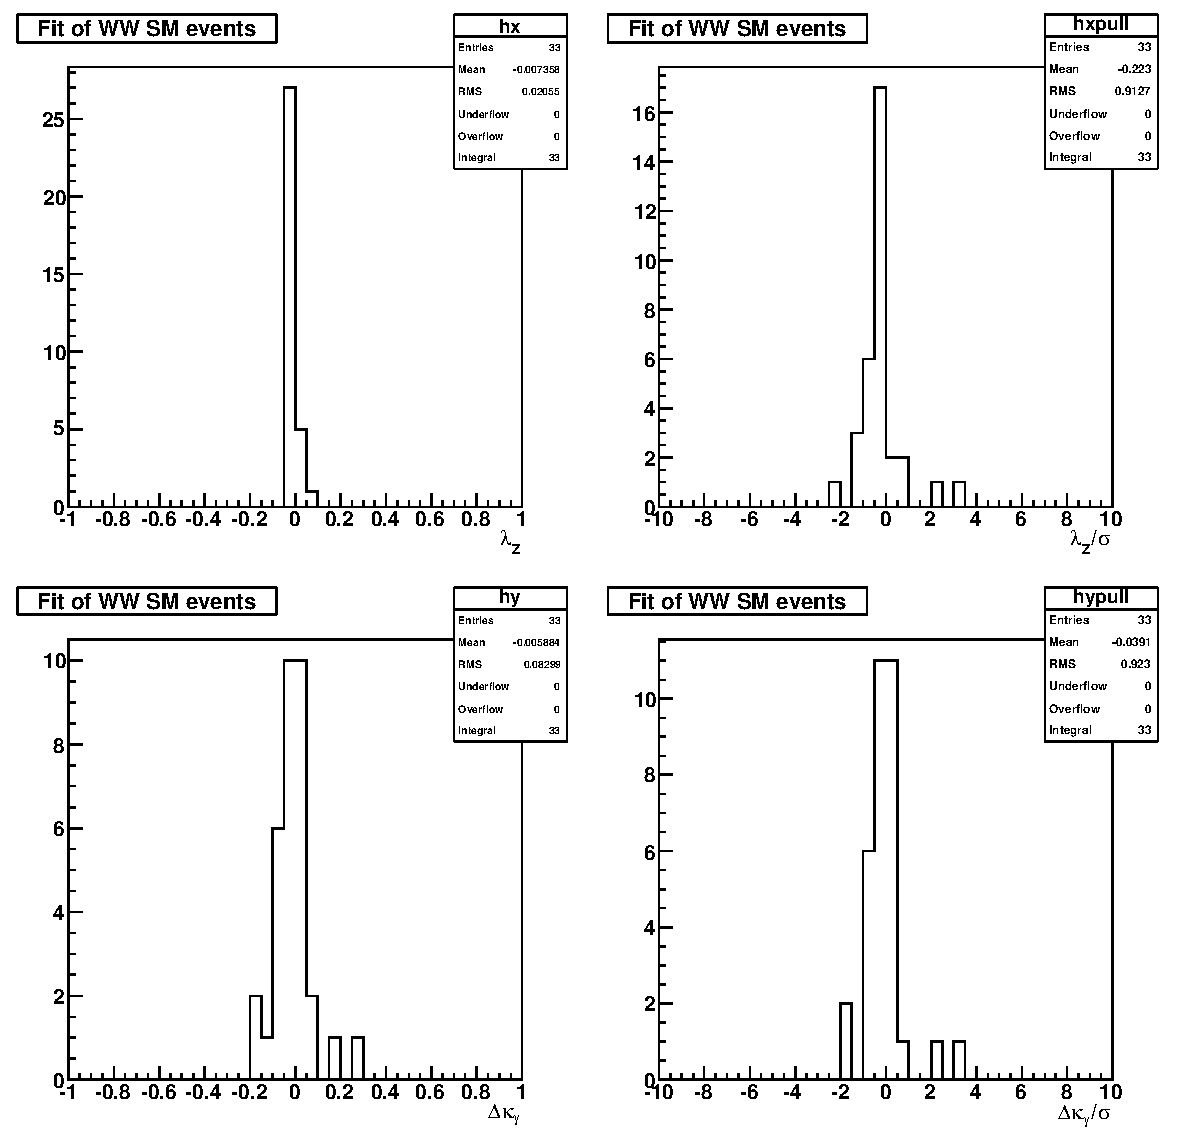
\includegraphics[width=1.0\textwidth]{figures/fit_ww_mc_1D_2}

  \caption[1D fits to WW SM Monte Carlo] {Fit results for
  2-dimentional $\lambda_{Z}$-$\Delta g^Z_1$ (top) and
  $\lambda_{Z}$-$\Delta\kappa_\gamma$ (bottom) aTGC models using 50
  independent pseudo-data experiments made of Madgraph Standard
  Model \ww\ simulated data. Only one coupling floating in the fit,
  while the other one is fixed to the Standard Model
  value. Backgrounds are excluded from the fits.}

\label{fig:fit_ww_mc_1D}
\end{figure}


%% \begin{figure}[tp]
%%   \centerline{
%%     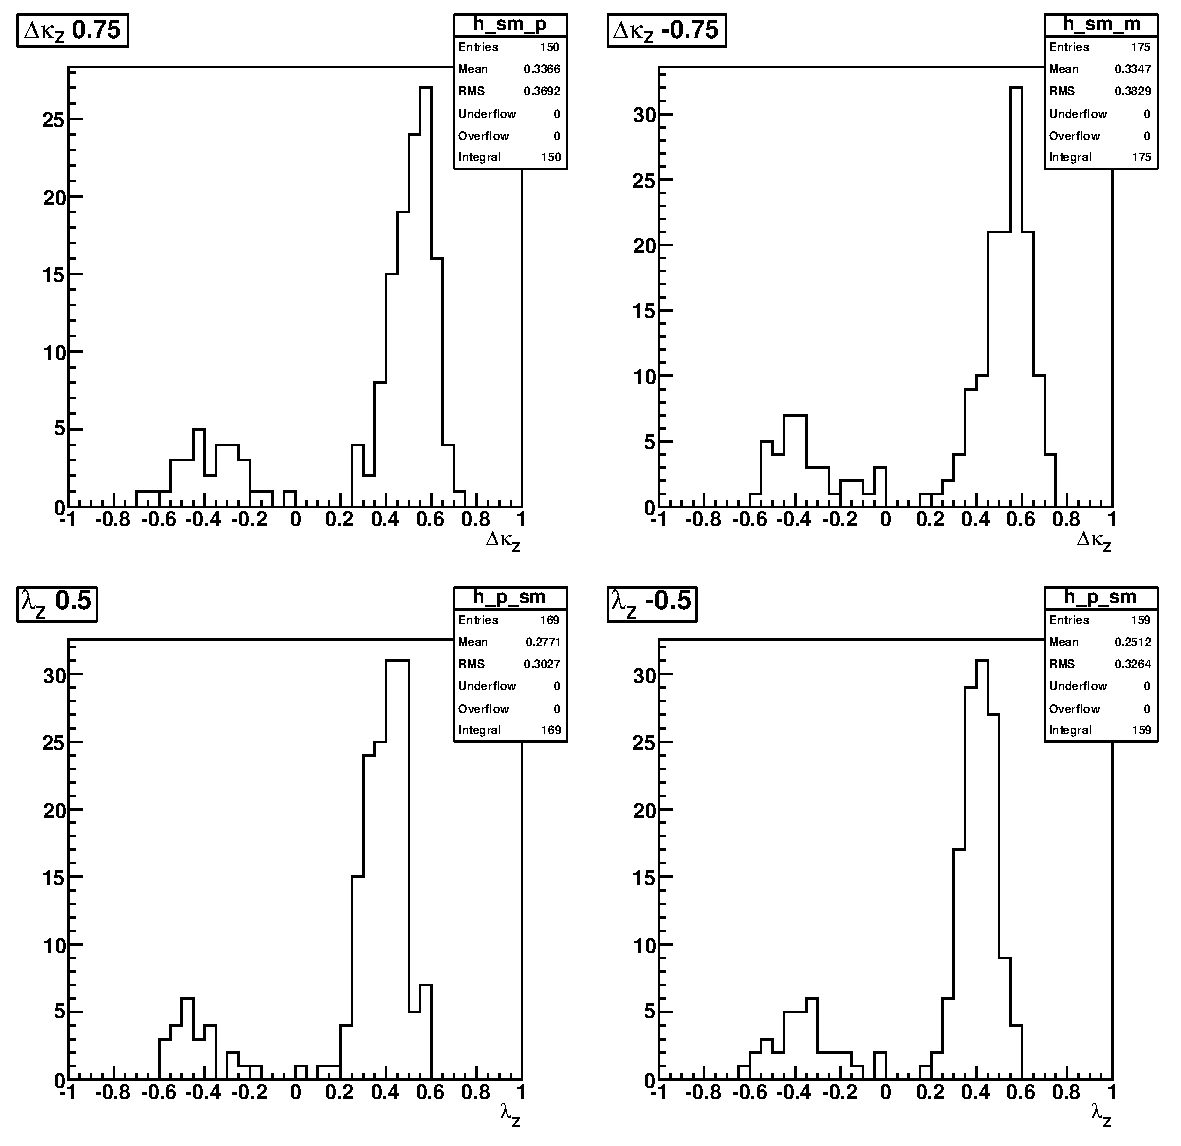
\includegraphics[width=1.0\textwidth]{figures/fit_wwATGC_mc_1D_pm}
%%   }

%%   \caption[1D fits to WW aTGC Monte Carlo] {Fits to WW Monte Carlo
%%     samples with anomalous couplings with 11 events in a sample. No
%%     background. Only one coupling is floated in the fit. Sign of the
%%     coupling cannot be determined in the fit.}
%%   \label{fig:fit_wwATGC_mc_1D_pm}
%% \end{figure}

\begin{figure}[tp]
  \centering
    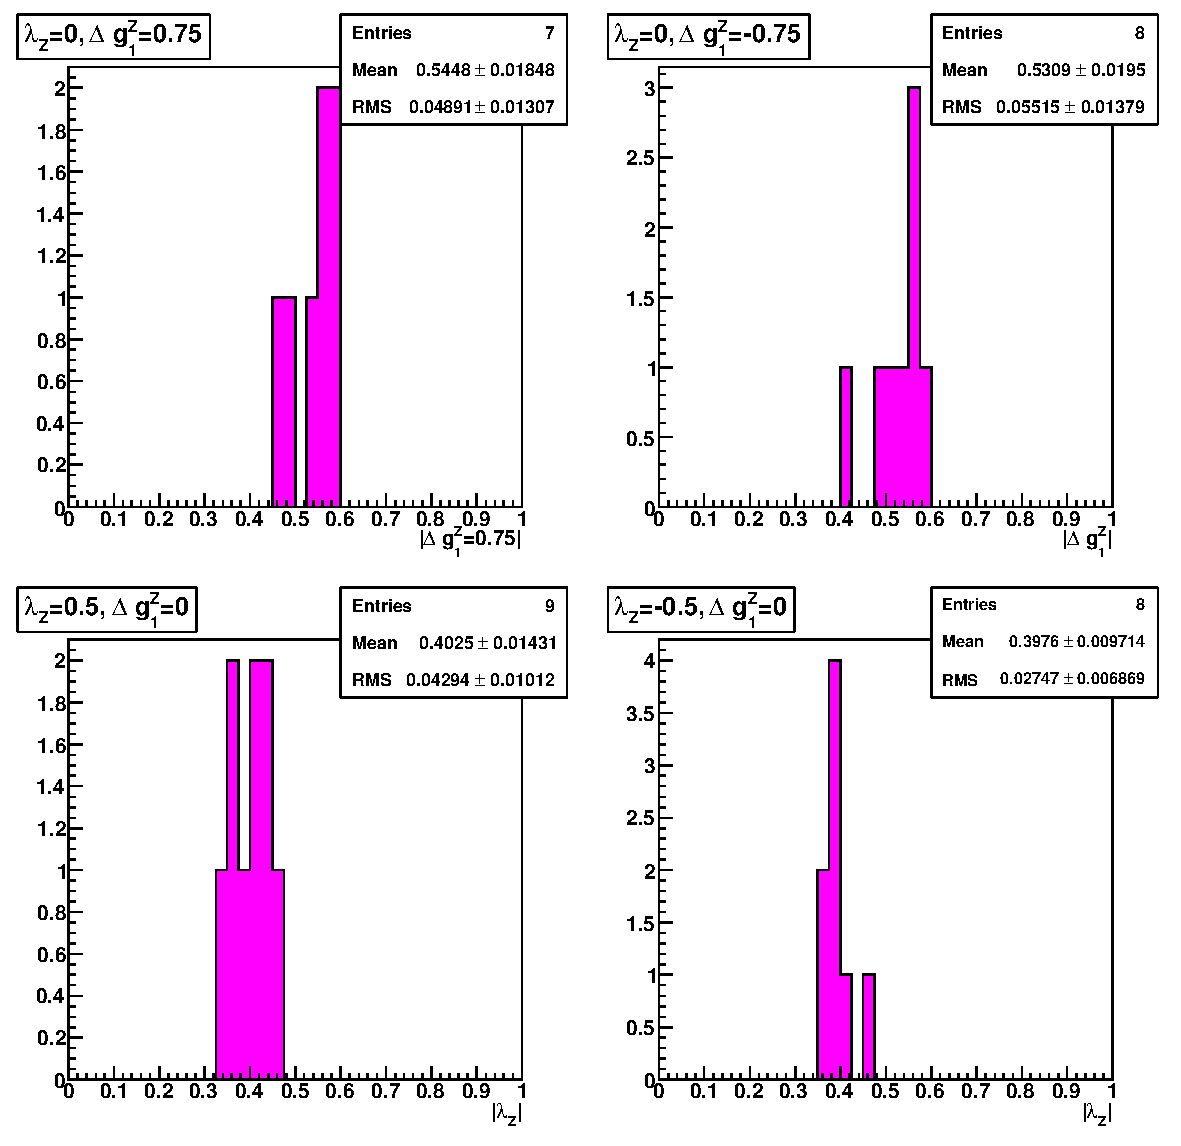
\includegraphics[width=0.8\textwidth]{figures/fit_wwATGC_mc_1D_abs}
    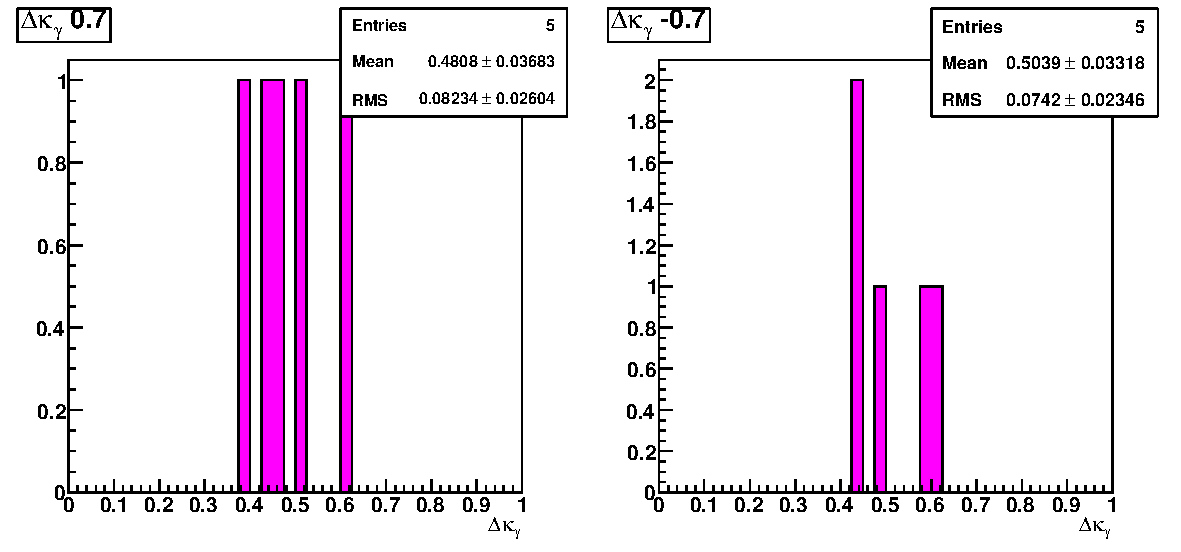
\includegraphics[width=0.8\textwidth]{figures/fit_wwATGC_mc_1D_abs2}

  \caption[1D fits to WW aTGC Monte Carlo] {Fits to $WW$ Monte Carlo
    samples with anomalous couplings. Pseudo-data experiments are made
    with 5-10 times lower number of events in each experiment due
    limited amount of simulated data. Backgrounds are excluded from
    the fits. Only one coupling is allowed to float in the
    fit. Absolute values of the couplings are  shown.}  
    \label{fig:fit_wwATGC_mc_1D_abs}
\end{figure}

\subsection{Fit on data}
We check how much the normalization of different components were
changed during the fit with respect to the inial values. For this test
we treat anomalous couplings as nuisance parameters and hide their
central values.

Table~\ref{tab:fit_yields} summarizes the fit results for event
yields. From it we conclude that the excess of the events that we
observed in the cross-section measurement is absorbed mostly in \wjets~
event yield. Looking at the correlation matrix
Figure~\ref{fig:fit_correlations} one can see that there is
significant correlation between \wjets~ and \ww~ event yields. Small
mis-modeling of the low pt part of the leading lepton distribution may
cause the excess to be split between the two contributions. This
effect has no impact on the anomalous coupling measurement, since it
mostly sensitive to the excess of events at high \pt{}.

%% Minuit2Minimizer: Minimize with max iterations 4000 edmval 1 strategy 1
%% Minuit2Minimizer : Valid minimum - status = 0
%% FVAL  = -1602.82913488348504
%% Edm   = 5.45511397378936264e-05
%% Nfcn  = 134
%% n_dy      = 15.9038    +/-  6.61673     (limited)
%% n_top     = 124.086    +/-  20.9979     (limited)
%% n_wjets   = 125.501    +/-  20.314      (limited)
%% n_ww      = 817.58     +/-  46.044      (limited)
%% n_wz      = 19.0359    +/-  1.89804     (limited)
%% n_zz      = 10.6562    +/-  0.999016    (limited)
%% x_par     = 0.00151822 +/-  0.0190978   (limited)
%% y_par     = 0.00503943 +/-  0.0304233   (limited)
%% Minos: Lower error for parameter 0  :  -6.74416
%% Minos: Upper error for parameter 0  :  6.74374
%% Minos: Lower error for parameter 1  :  -20.8847
%% Minos: Upper error for parameter 1  :  21.2024
%% Minos: Lower error for parameter 2  :  -20.2856
%% Minos: Upper error for parameter 2  :  20.4984
%% Minos: Lower error for parameter 3  :  -46.2509
%% Minos: Upper error for parameter 3  :  45.9041
%% Minos: Lower error for parameter 4  :  -1.89954
%% Minos: Upper error for parameter 4  :  1.89966
%% Minos: Lower error for parameter 5  :  -0.999735
%% Minos: Upper error for parameter 5  :  0.999722
%% Minos: Lower error for parameter 6  :  -0.0189644
%% Minos: Upper error for parameter 6  :  0.0182371
%% Minos: Lower error for parameter 7  :  -0.0301162
%% Minos: Upper error for parameter 7  :  0.0295189
%%
%%   RooFitResult: minimized FCN value: -1602.83, estimated distance to minimum: 2.12194e-05
%%                 covariance matrix quality: Full, accurate covariance matrix
%%
%%     Floating Parameter  InitialValue    FinalValue +/-  Error     GblCorr.
%%   --------------------  ------------  --------------------------  --------
%%                   n_dy    1.5909e+01    1.5909e+01 +/-  6.62e+00  0.215534
%%                  n_top    1.2416e+02    1.2416e+02 +/-  2.10e+01  0.522827
%%                n_wjets    1.2557e+02    1.2557e+02 +/-  2.03e+01  0.547777
%%                   n_ww    8.1733e+02    8.1733e+02 +/-  4.61e+01  0.687014
%%                   n_wz    1.9036e+01    1.9036e+01 +/-  1.90e+00  0.063578
%%                   n_zz    1.0656e+01    1.0656e+01 +/-  9.99e-01  0.031781
%%                  x_par    1.5155e-03    1.5155e-03 +/-  1.91e-02  0.113013
%%                  y_par    5.0221e-03    5.0221e-03 +/-  3.04e-02  0.121154


\begin{table}[!ht]
  \begin{center}
 {\small
  \begin{tabular} {|l|c|c|c|}
\hline
  Parameter       &   Initial value & Fit value & Global Correlation \\
\hline
  N$_{\ww}$       & $819.9\pm57.6$  & $817.6\pm46.0$ & 0.69 \\
  N$_{Top}$       & $121.6\pm23.4$  & $124.1\pm21.0$ & 0.52 \\
  N$_{\wjets}$    & $78.1\pm22.0$   & $125.6\pm20.3$ & 0.55 \\
  N$_{\wz}$       & $18.5\pm1.9$    & $19.0\pm1.9$   & 0.06 \\
  N$_{\dyll}$     & $11.7\pm6.8$    & $15.9\pm6.6$   & 0.22 \\
  N$_{\zz}$       & $10.6\pm1.0$    & $10.7\pm1.0$   & 0.03 \\
\hline
  \end{tabular}
  }
  \caption{Nominal fit parameter values.}
   \label{tab:fit_yields}
  \end{center}
\end{table}

\begin{figure}[tp]
  \centerline{
    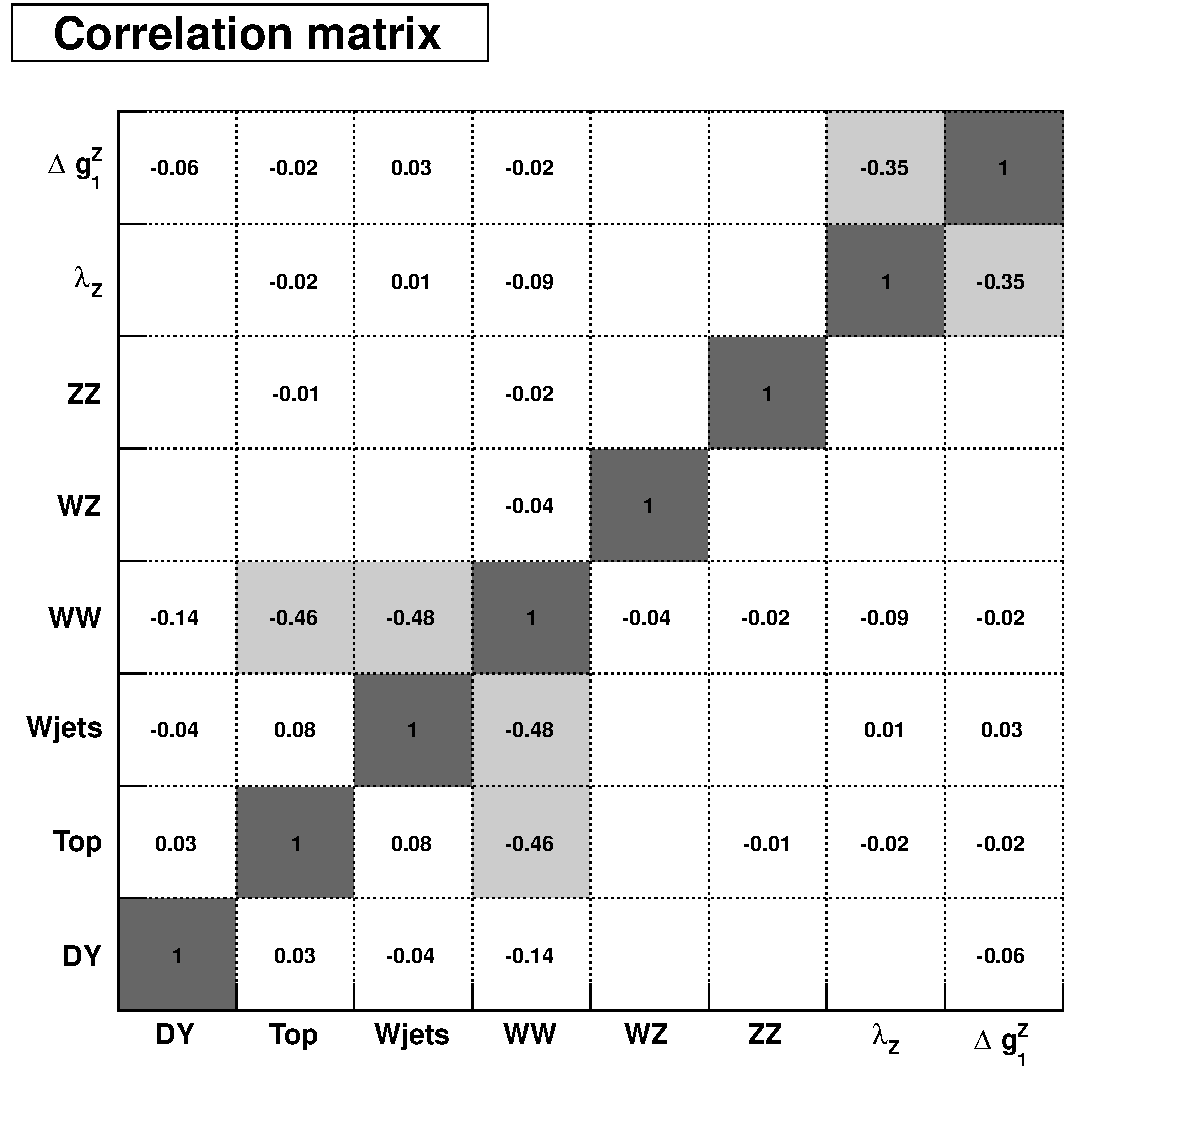
\includegraphics[width=.45\textwidth]{figures/correlations}
  }

  \caption[Fit parameter correlations] {Correlation matrix for the nominal fit parameters.}
  \label{fig:fit_correlations}
\end{figure}
